%% abtex2-modelo-slides.tex, v-1.0 gfabinhomat
%% Copyright 2012-2015 by abnTeX2 group at http://www.abntex.net.br/ 
%%
%% This work may be distributed and/or modified under the
%% conditions of the LaTeX Project Public License, either version 1.3
%% of this license or (at your option) any later version.
%% The latest version of this license is in
%%   http://www.latex-project.org/lppl.txt
%% and version 1.3 or later is part of all distributions of LaTeX
%% version 2005/12/01 or later.
%%
%% This work has the LPPL maintenance status `maintained'.
%% 
%% The Current Maintainer of this work is Fábio Rodrigues Silva, 
%% member of abnTeX2 team, led by Lauro César Araujo. 
%% Further information are available on 
%% http://www.abntex.net.br/
%%
%% This work consists of the files abntex2-modelo-slides.tex, 
%% abntex2-modelo-references.bib and abntex2-modelo-marca.pdf
%%
%% Modelo desenvolvido por Fábio Rodrigues Silva (gfabinhomat@gmail.com)
%% Mais informações podem ser obtidas no guia do usuário Beamer 
%% (http://linorg.usp.br/CTAN/macros/latex/contrib/beamer/doc/beameruserguide.pdf)
%% Informações rápidas podem ser acessadas em http://en.wikibooks.org/wiki/LaTeX/Presentations


% Apresentações em widescreen. Outros valores possíveis: 1610, 149, 54, 43 e 32.
% Por padrão, as apresentações são no formato 4:3 (sem o aspectratio).
\documentclass[aspectratio=169]{beamer}	 	

\usetheme{Berlin}
\usecolortheme{dolphin}
\usefonttheme[onlymath]{serif}			% para fontes matemáticas
% Enconte mais temas e cores em http://www.hartwork.org/beamer-theme-matrix/ 
% Veja também http://deic.uab.es/~iblanes/beamer_gallery/index.html

% Customizações de Cores: fg significa cor do texto e bg é cor do fundo
% ---
% PACOTES
% ---
\usepackage[alf]{abntex2cite}		% Citações padrão ABNT
\usepackage[brazil]{babel}		% Idioma do documento
\usepackage{color}			% Controle das cores
\usepackage[T1]{fontenc}		% Selecao de codigos de fonte.
\usepackage{graphicx}			% Inclusão de gráficos
\usepackage[utf8]{inputenc}		% Codificacao do documento (conversão automática dos acentos)
\usepackage{txfonts}			% Fontes virtuais
% ---
\usepackage{caption}
% --- Informações do documento ---
\title{Identificação de Parâmetros através de Sinal Persistentemente Excitante com Esquema de Desligamento Automático}
\author{Pedro Yochinori Gushiken\\ Orientador: Aldayr Dantas de Araújo}
\institute{Universidade Federal do Rio Grande do Norte}
\date{\today}
% ---

% ----------------- INÍCIO DO DOCUMENTO --------------------------------------
\begin{document}

% ----------------- NOVO SLIDE --------------------------------
\begin{frame}

\begin{minipage}{1\linewidth}
  \centering
\end{minipage}

\titlepage

\end{frame}

% ----------------- NOVO SLIDE --------------------------------
\begin{frame}{Sumário}
\tableofcontents
\end{frame}

% ----------------- NOVO SLIDE --------------------------------
\section{Introdução}
\begin{frame}
\frametitle{Contextualização}
\begin{enumerate}
\item<1-> Controle de Processos\\
\item<2-> Identificação de Parâmetros\\ 
\item<3-> Perturbação e Persistência de Excitação\\
\item<4-> Robustez\\
\item<5-> Desempenho\\
\end{enumerate}
\end{frame}


% ----------------- NOVO SLIDE --------------------------------
\section{Preparação}
\subsection{Plantas Estudadas}
\begin{frame}
\frametitle{Funções de Transferência}
\begin{equation}
G_1(s)=\frac{A}{\tau s+1}
\end{equation}
\begin{equation}
A=0.0833;~\tau=0.00833
\end{equation}

Onde (1) e (2) são referentes à Planta de Primeira Ordem

\begin{equation}
G_2(s) = \frac{A}{(\tau_1 s + 1)(\tau_2 s + 1)}
\end{equation}
\begin{equation}
A=0.195;~\tau_1=0.1;~\tau_2=0.05
\end{equation}

Onde (3) e (4) são referentes à Planta de Segunda Ordem

\end{frame}
\begin{frame}
\frametitle{EDOs}
\begin{equation}
\dot{y} = 100u(t) - 120y(t)
\end{equation}

Onde (5) é a EDO referente à Planta de Primeira Ordem

\begin{equation}
\ddot{y}= 39u(t) - 200y(t) - 30\dot{y}(t)
\end{equation}

Onde (6) é a EDO referente à Planta de Segunda Ordem 

\end{frame}
\subsection{Conceitos}
\begin{frame}
\frametitle{Método do Gradiente com Regra de Ajuste do MIT}

\begin{equation}
\dot{\hat{y}} = \hat{\theta_1}u-\hat{\theta_2}\hat{y}
\end{equation}
\begin{equation}
\dot{\hat{\theta_1}} = \gamma_1e_0u
\end{equation}
\begin{equation}
\dot{\hat{\theta_2}} = -\gamma_2e_0\hat{y}
\end{equation}

Onde (7) é a EDO referente ao modelo da planta e (8) e (9) as equações referentes à adaptação das estimativas dos parâmetros.

\end{frame}

\begin{frame}
\frametitle{Método do Gradiente com Regra de Ajuste do MIT}

\begin{equation}
\ddot{\hat{y}} = \hat{\theta_1}u-\hat{\theta_2}\hat{y}- \hat{\theta_3}\dot{\hat{y}}
\end{equation}
\begin{equation}
\dot{\hat{\theta_1}} = \gamma_1e_0u
\end{equation}
\begin{equation}
\dot{\hat{\theta_2}} = -\gamma_2e_0\hat{y}
\end{equation}
\begin{equation}
\dot{\hat{\theta_3}} = -\gamma_2e_0\dot{\hat{y}}
\end{equation}


Onde (10) é a EDO referente ao modelo da planta de segunda ordem e (11) e (12) e (13) as equações referentes à adaptação das estimativas dos parâmetros.

\end{frame}

\begin{frame}
\frametitle{Característica de Persistência de Excitação de um Sinal}

 Um sinal $u:\mathcal{R}^+\rightarrow \mathcal{R}$ é dito suficientemente rico em frequências de ordem n se contiver pelo menos n/2 frequências distintas.\\

 Um sinal $\phi = H(s)u $ é persistentemente excitante se e somente se $u$ é um sinal rico em frequências de ordem n e estacionário com $H(jw_1),...,H(jw_n)$ linearmente independentes em $C^n$ para todo $w_1,...,w_n \in R$ onde $w_i\neq w_k$ para $i\neq k$. \\

\end{frame}
\begin{frame}
\frametitle{Esquema de Desligamento do Sinal PE}
Definimos a matriz: \[
Q=
  \begin{bmatrix}
    1/q_1^2 & 0       &  0       &  ... &  0      \\
    0       & 1/q_2^2 &  0       &  ... &  0      \\
    0       & 0       &  1/q_3^2 &  ... &  0      \\
    ...     & ...     &  ...     &      &  ...    \\
    0       & 0       &  0       &  ... & 1/q_n^2
  \end{bmatrix}
\]

Que é usada na seguinte equação:

\begin{equation}
\varepsilon = \frac{\dot{\hat{\theta}}^TQ\dot{\hat{\theta}}}{\dot{\hat{\theta}}^TQ\dot{\hat{\theta}}+1}
\end{equation}

\end{frame}

\begin{frame}
\frametitle{Esquema de Desligamento do Sinal PE}
Temos que $0\leq\varepsilon<1$ e a partir desta figura de mérito geramos o seguinte sinal a ser introduzido na planta:
  \begin{align*}
      r &= q(t) + r_0 ; & \varepsilon > L  \\
      r &= r_0 ; & \varepsilon \leq L
  \end{align*}

Onde escolhemos $L=0.5$ e $q(t)$ é uma onda quadrada, que pela definição usada contém a característica de ser PE.

\end{frame}

\subsection{Diagrama das Simulações}
\begin{frame}
\frametitle{Planta de Primeira Ordem}

\centering
\begin{minipage}{.48\textwidth}
  \centering
  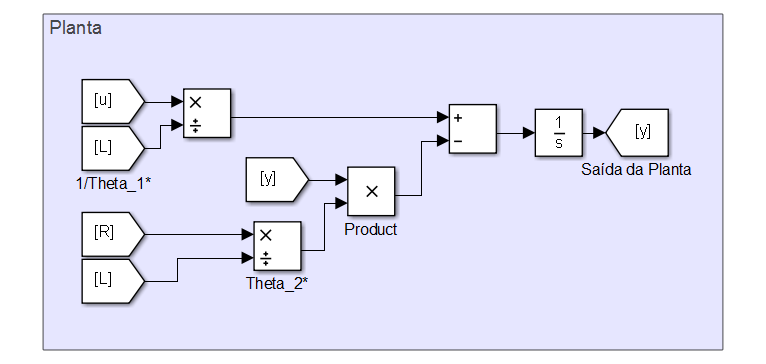
\includegraphics[width=\linewidth]{./pics/PlantaPrimeiraOrdemSemZeroPlanta.png}
  \captionof{figure}{Planta de Primeira Ordem}
  \label{fig:test23}
\end{minipage}%
  \hfill
\begin{minipage}{.48\textwidth}
  \centering
  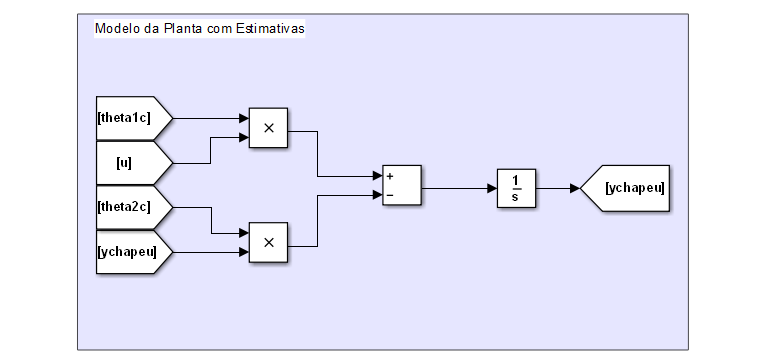
\includegraphics[width=\linewidth]{./pics/PlantaPrimeiraOrdemSemZeroModeloPlanta.png}
  \captionof{figure}{Modelo da Planta de Primeira Ordem}
  \label{fig:test24}
\end{minipage}
\end{frame}
\begin{frame}
\frametitle{Planta de Primeira Ordem}

\centering
\begin{minipage}{.48\textwidth}
  \centering
  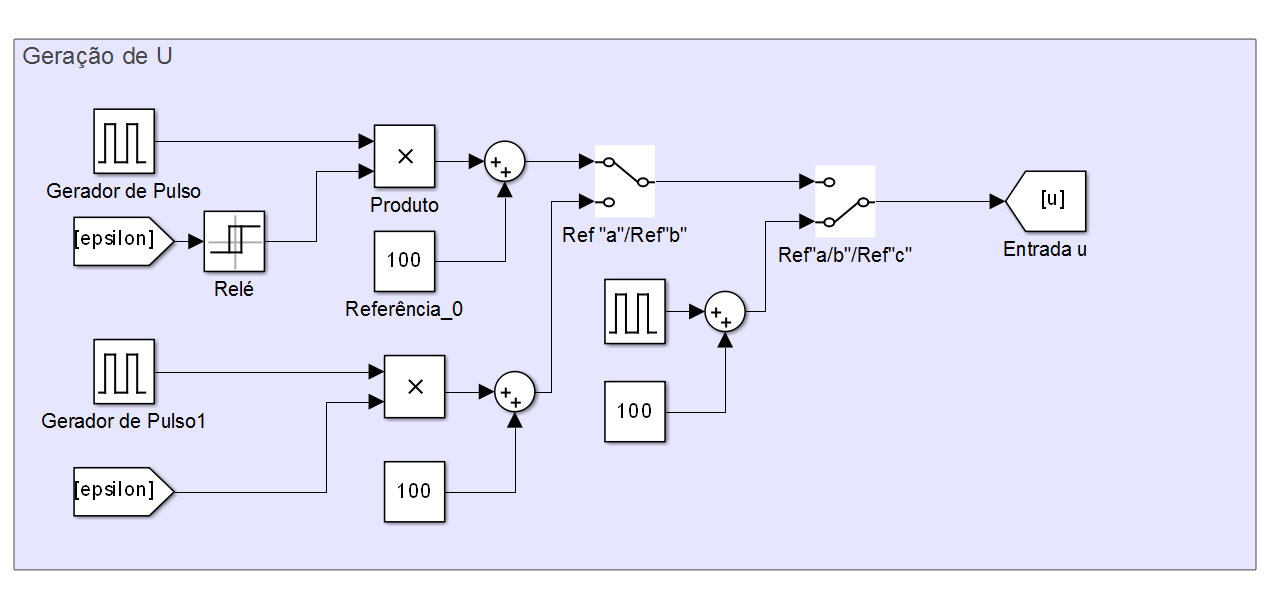
\includegraphics[width=\linewidth]{./pics/PlantaPrimeiraOrdemSemZeroU.png}
  \captionof{figure}{Geração do Sinal de Entrada}
  \label{fig:test25}
\end{minipage}%
  \hfill
\begin{minipage}{.48\textwidth}
  \centering
  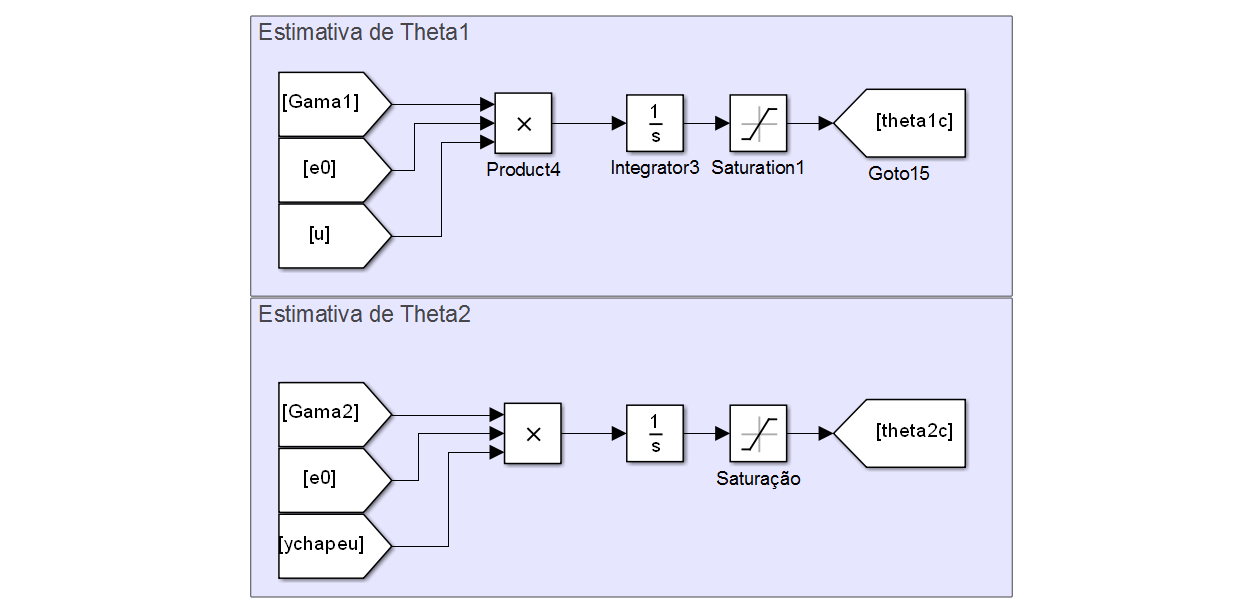
\includegraphics[width=\linewidth]{./pics/PlantaPrimeiraOrdemSemZeroEstimativas.png}
  \captionof{figure}{Geração das Estimativas dos Parâmetros da Planta}
  \label{fig:test26}
\end{minipage}
\end{frame}
\begin{frame}
\frametitle{Planta de Primeira Ordem}
  \centering
  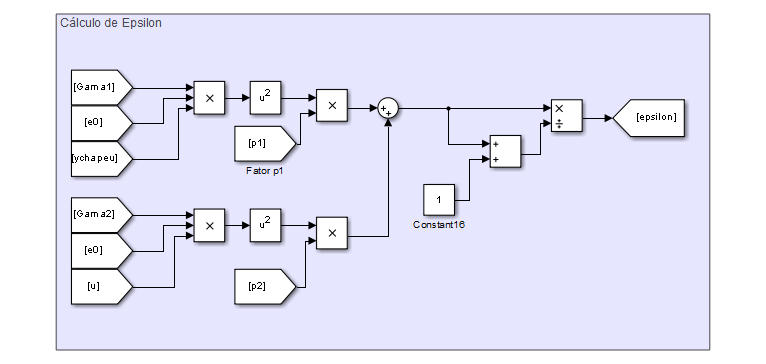
\includegraphics[width=.5\linewidth]{./pics/PlantaPrimeiraOrdemSemZeroEpsilon.png}
  \captionof{figure}{Cálculo de $\varepsilon$}
  \label{fig:test30}
\end{frame}
\begin{frame}
\frametitle{Planta de Segunda Ordem}
\centering
\begin{minipage}{.48\textwidth}
  \centering
  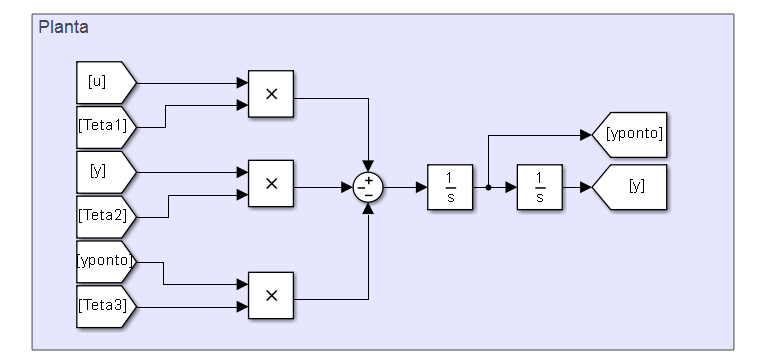
\includegraphics[width=\linewidth]{./pics/PlantaSegundaOrdemPlanta.png}
  \captionof{figure}{Planta de Segunda Ordem}
  \label{fig:test31}
\end{minipage}%
  \hfill
\begin{minipage}{.48\textwidth}
  \centering
  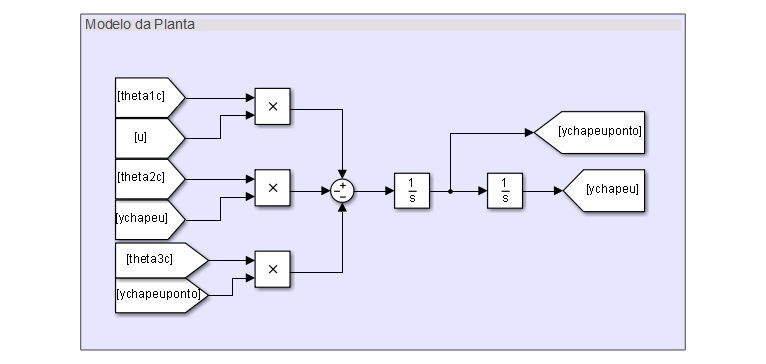
\includegraphics[width=\linewidth]{./pics/PlantaSegundaOrdemModeloPlanta.png}
  \captionof{figure}{Modelo da Planta de Segunda Ordem}
  \label{fig:test41}
\end{minipage}
\end{frame}
\begin{frame}
\frametitle{Planta de Segunda Ordem}
\centering
\begin{minipage}{.48\textwidth}
  \centering
  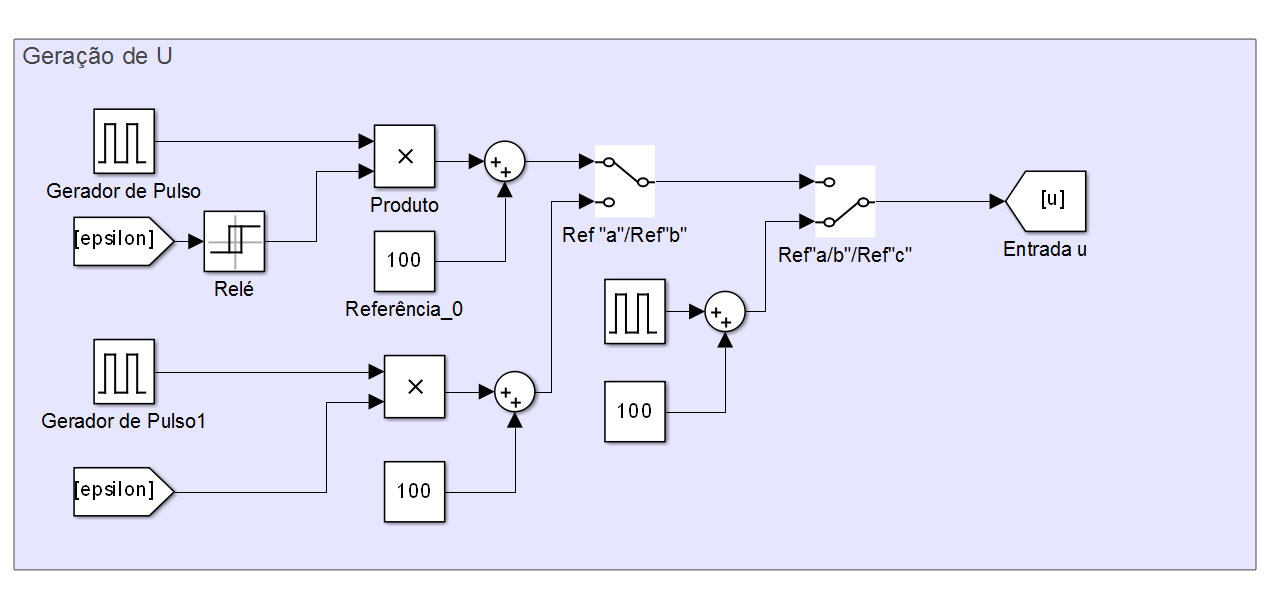
\includegraphics[width=\linewidth]{./pics/PlantaSegundaOrdemU.png}
  \captionof{figure}{Geração do Sinal de Entrada}
  \label{fig:test32}
\end{minipage}%
  \hfill
\begin{minipage}{.48\textwidth}
  \centering
  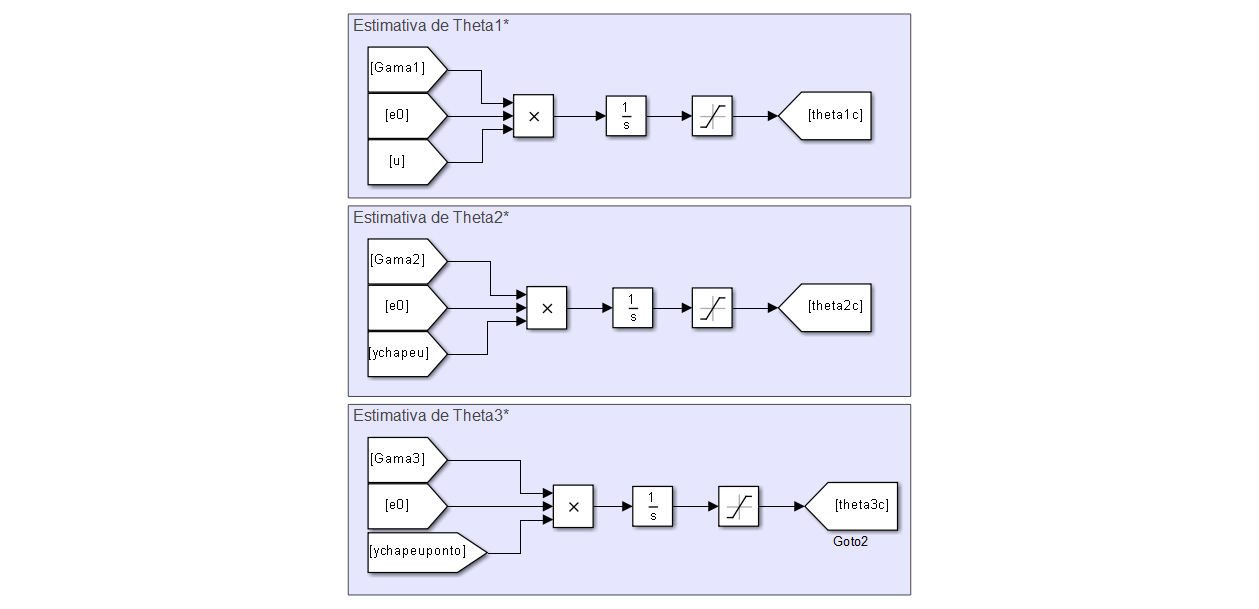
\includegraphics[width=\linewidth]{./pics/PlantaSegundaOrdemEstimativas.png}
  \captionof{figure}{Geração das Estimativas dos Parâmetros da Planta}
  \label{fig:test43}
\end{minipage}
\end{frame}
\begin{frame}
\frametitle{Planta de Segunda Ordem}
  \centering
  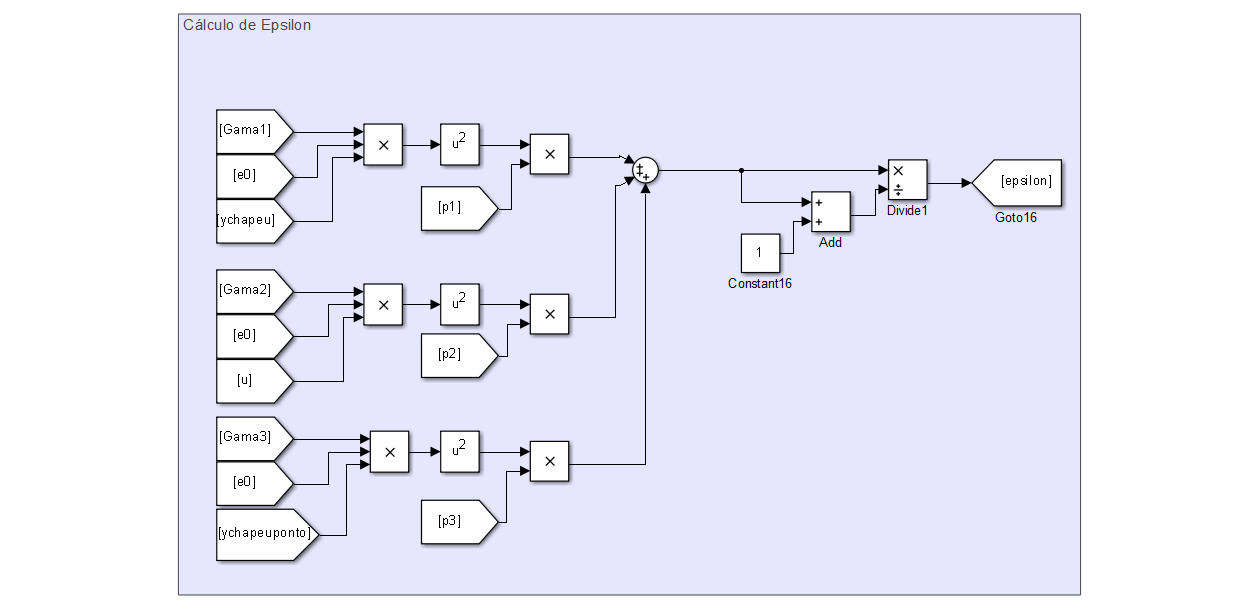
\includegraphics[width=.5\linewidth]{./pics/PlantaSegundaOrdemEpsilon.png}
  \captionof{figure}{Cálculo do valor de $\varepsilon$}
  \label{fig:test340}
\end{frame}






% ----------------- NOVO SLIDE --------------------------------
\section{Resultados}
\subsection{Planta de Primeira Ordem}

% % % % % % % % % % % % % % % % %REF C
\begin{frame}
\frametitle{Sinal introduzido na Planta e Saída da Planta}
\centering
\begin{minipage}{.48\textwidth}
  \centering
  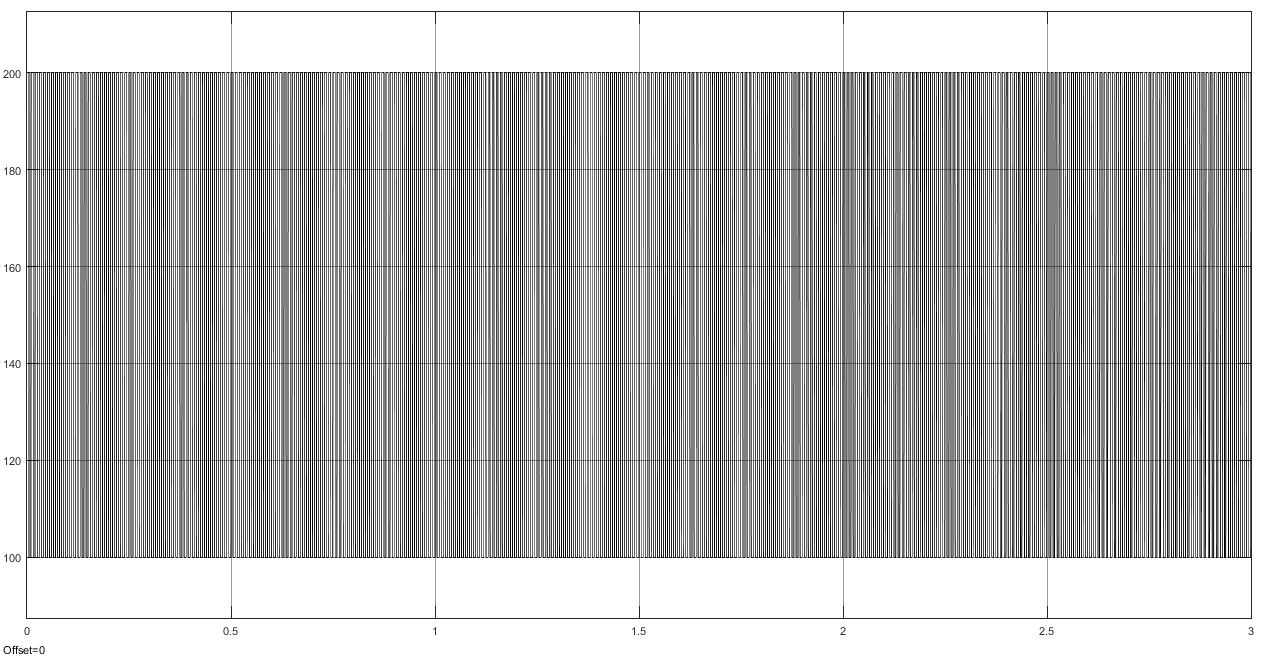
\includegraphics[width=\linewidth]{./pics/EntradaU.png}
  \captionof{figure}{Sinal Introduzido na Planta, Referência PE para todo t}
  \label{fig:test3}
\end{minipage}%
  \hfill
\begin{minipage}{.48\textwidth}
  \centering
  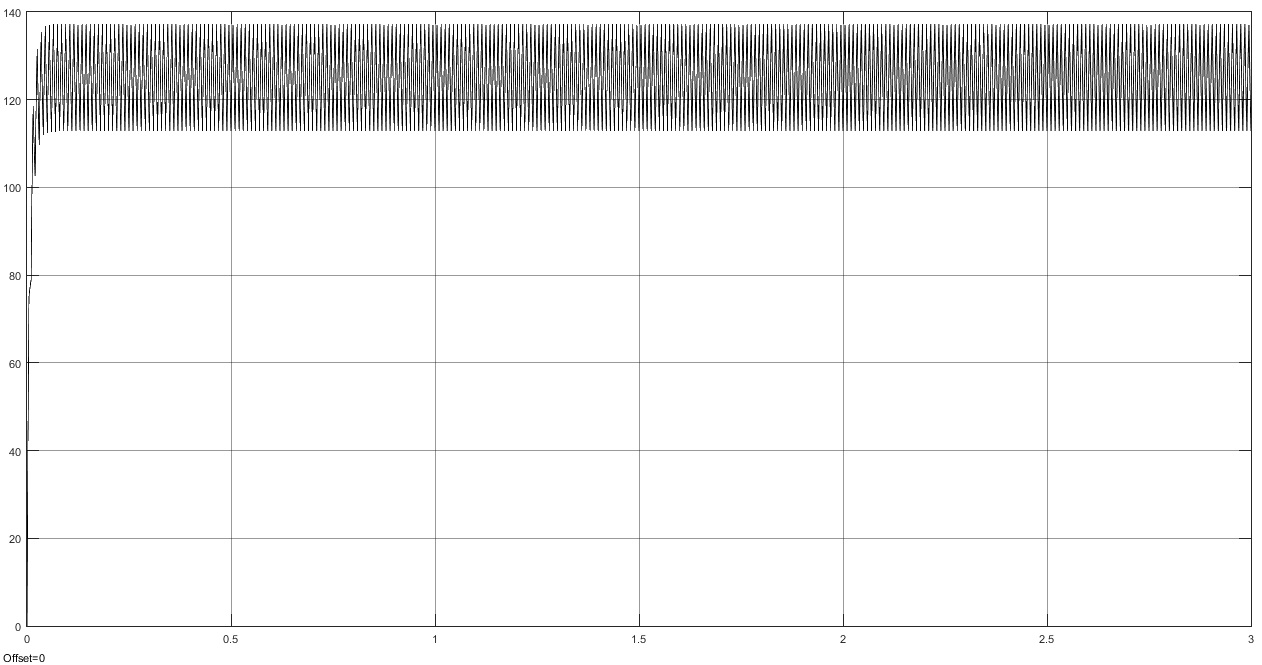
\includegraphics[width=\linewidth]{./pics/ResultadoPrimeiraOrdemEstimativaYRefC.png}
  \captionof{figure}{Saída da Planta, Referência PE para todo t}
  \label{fig:test4}
\end{minipage}
\end{frame}
\begin{frame}
\frametitle{Saída do Modelo da Planta e Erro de Saída}
\centering
\begin{minipage}{.48\textwidth}
  \centering
  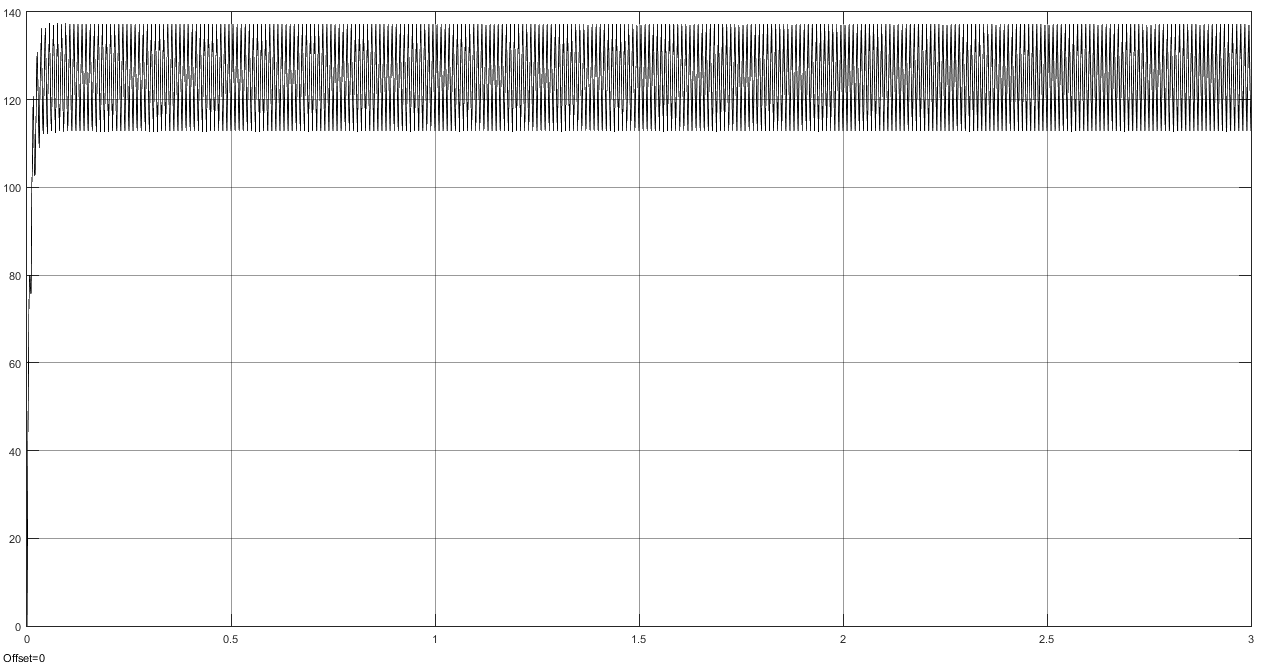
\includegraphics[width=\linewidth]{./pics/ResultadoPrimeiraOrdemEstimativaYcRefC.png}
  \captionof{figure}{Saída do Modelo da Planta, Referência PE para todo t}
  \label{fig:test5}
\end{minipage}%
  \hfill
\begin{minipage}{.48\textwidth}
  \centering
  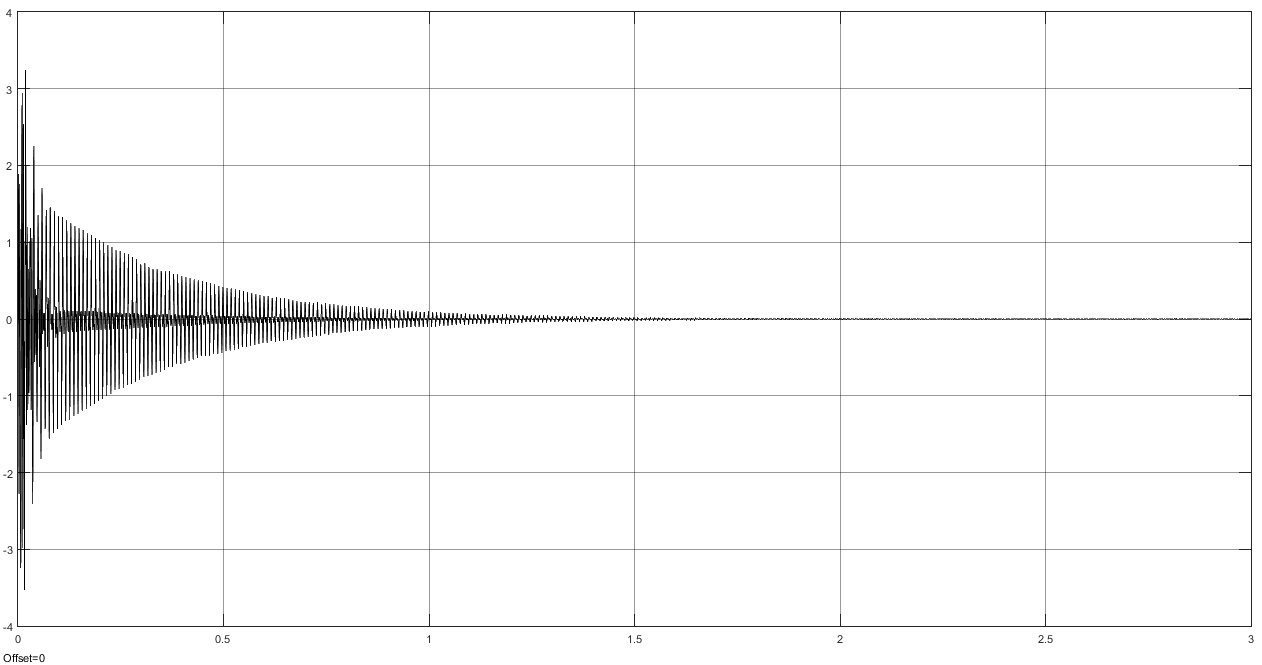
\includegraphics[width=\linewidth]{./pics/ResultadoPrimeiraOrdemEstimativaE0RefC.png}
  \captionof{figure}{Erro de Saída da Planta, Referência PE para todo t}
  \label{fig:test6}
\end{minipage}
\end{frame}
\begin{frame}
\frametitle{Estimativas dos Parâmetros da Planta}
\centering
\begin{minipage}{.48\textwidth}
  \centering
  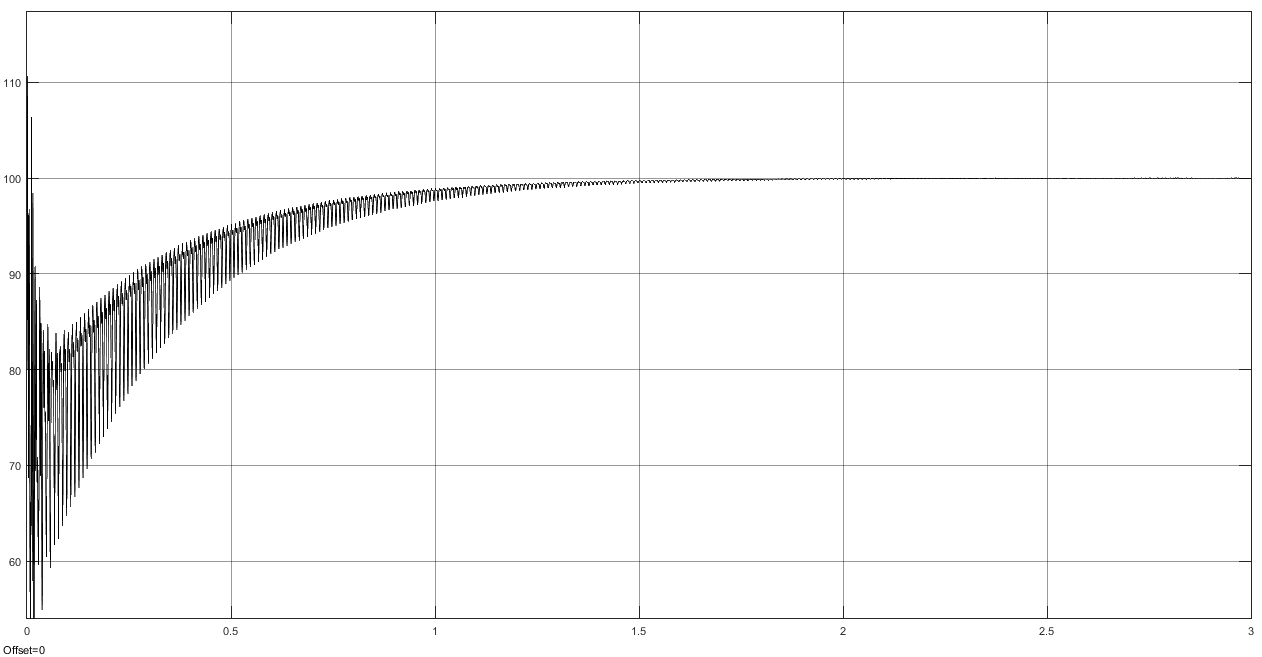
\includegraphics[width=\linewidth]{./pics/ResultadoPrimeiraOrdemEstimativaTheta1RefC.png}
  \captionof{figure}{Estimativa $\hat{\theta_1}$, $\theta_1^*=100$, Referência PE para todo t}
  \label{fig:test7}
\end{minipage}%
  \hfill
\begin{minipage}{.48\textwidth}
  \centering
  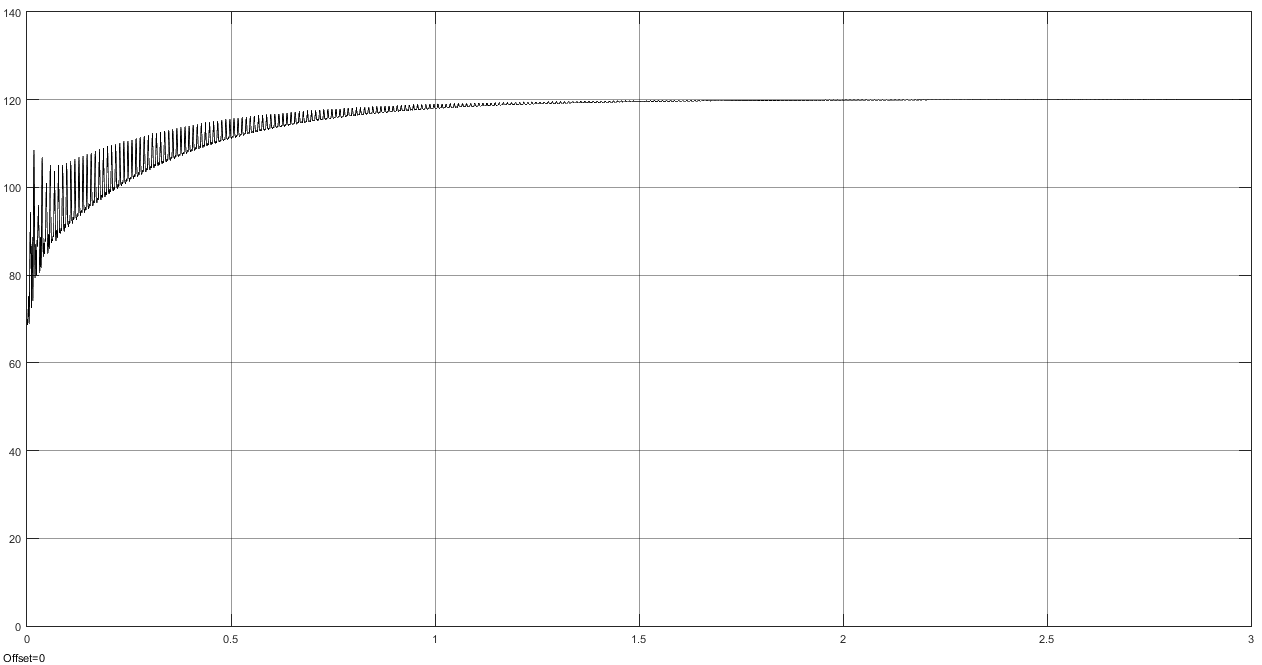
\includegraphics[width=\linewidth]{./pics/ResultadoPrimeiraOrdemEstimativaTheta2RefC.png}
  \captionof{figure}{Estimativa $\hat{\theta_2}$, $\theta_2^*=120$, Referência PE para todo t}
  \label{fig:test8}
\end{minipage}
\end{frame}
% % % % % % % % % % % % % % % % % % % % % % % % %REF A

\begin{frame}
\frametitle{Sinal introduzido na Planta e Saída da Planta}
\centering
\begin{minipage}{.48\textwidth}
  \centering
  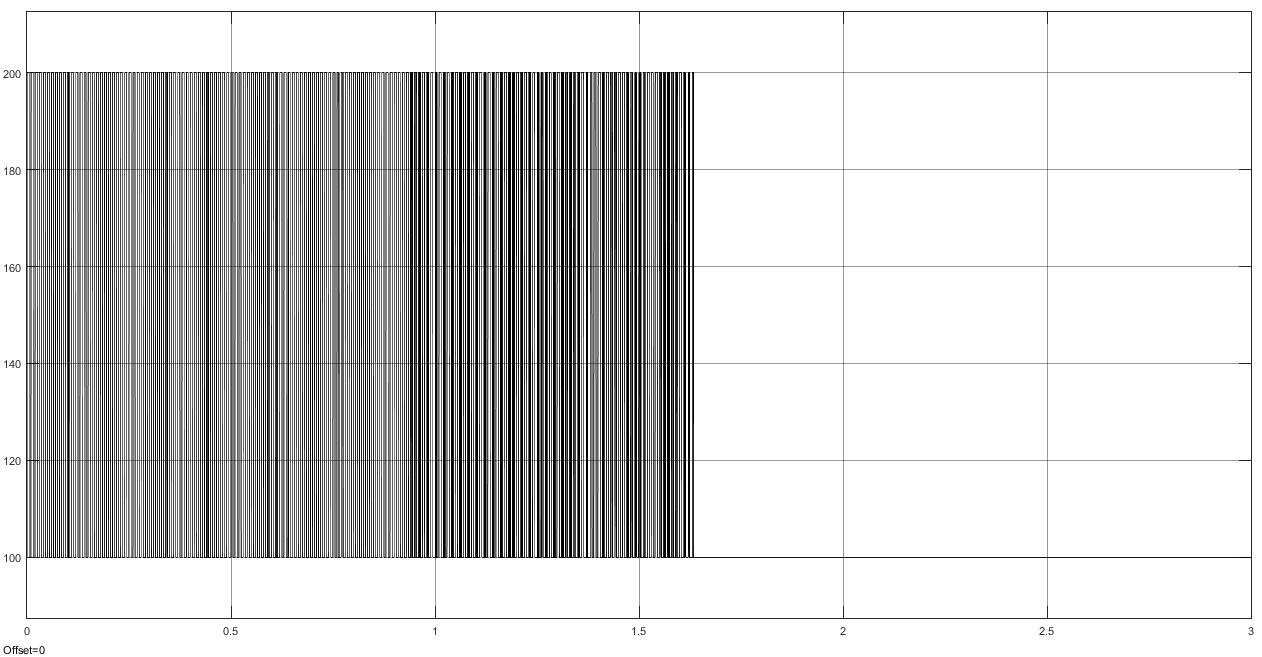
\includegraphics[width=\linewidth]{./pics/EntradaURefA.png}
  \captionof{figure}{Sinal Introduzido na Planta, Referência PE um tempo finito}
  \label{fig:test37}
\end{minipage}%
  \hfill
\begin{minipage}{.48\textwidth}
  \centering
  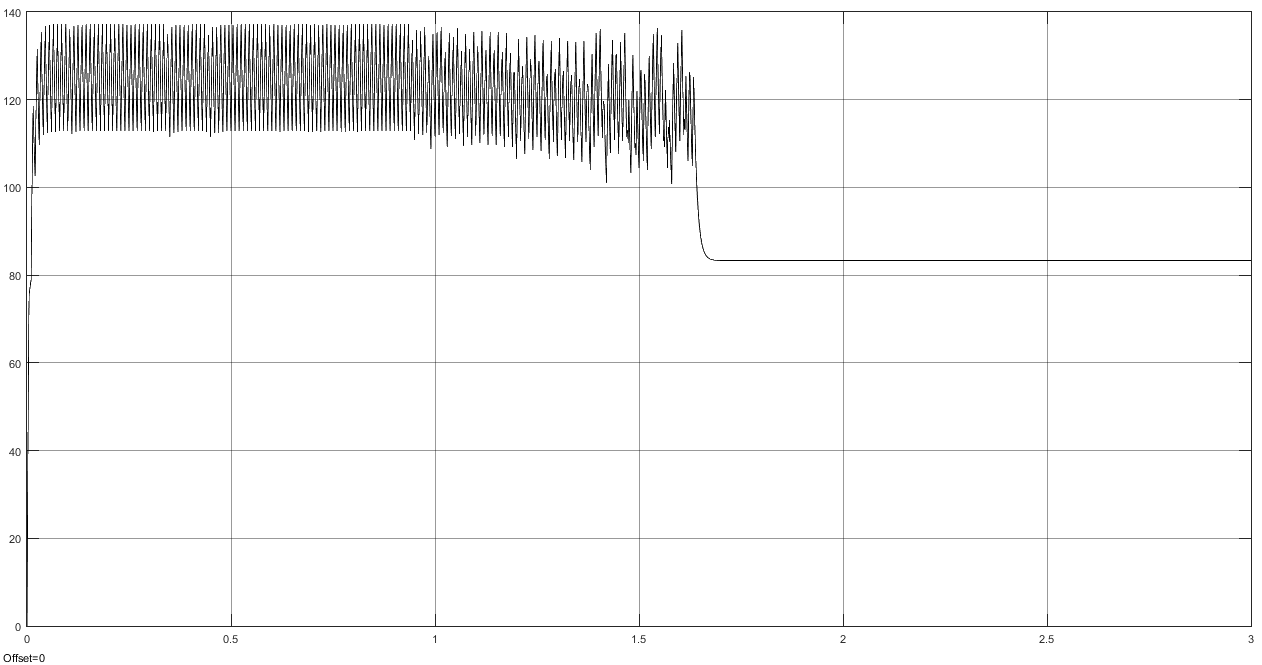
\includegraphics[width=\linewidth]{./pics/ResultadoPrimeiraOrdemEstimativaYRefA.png}
  \captionof{figure}{Saída da Planta, Referência PE para um tempo finito}
  \label{fig:test40}
\end{minipage}
\end{frame}
\begin{frame}
\frametitle{Saída do Modelo da Planta e Erro de Saída}
\centering
\begin{minipage}{.48\textwidth}
  \centering
  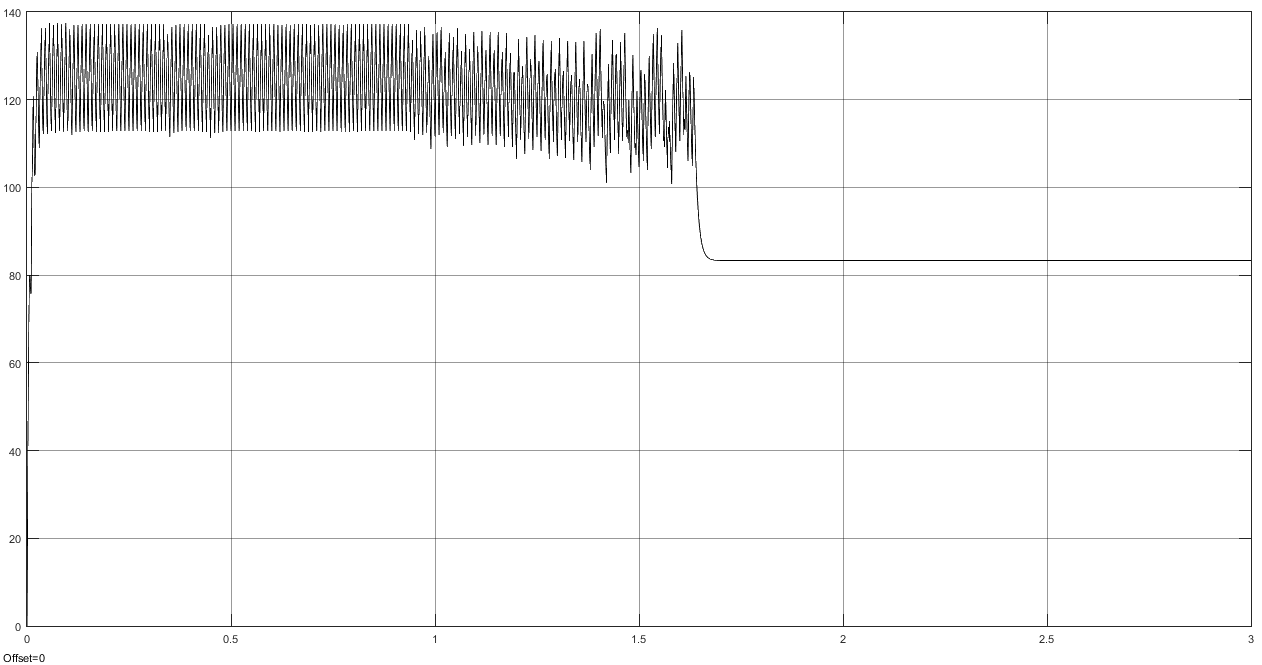
\includegraphics[width=\linewidth]{./pics/ResultadoPrimeiraOrdemEstimativaYcRefA.png}
  \captionof{figure}{Saída do Modelo da Planta, Referência PE para um tempo finito}
  \label{fig:test50}
\end{minipage}%
  \hfill
\begin{minipage}{.48\textwidth}
  \centering
  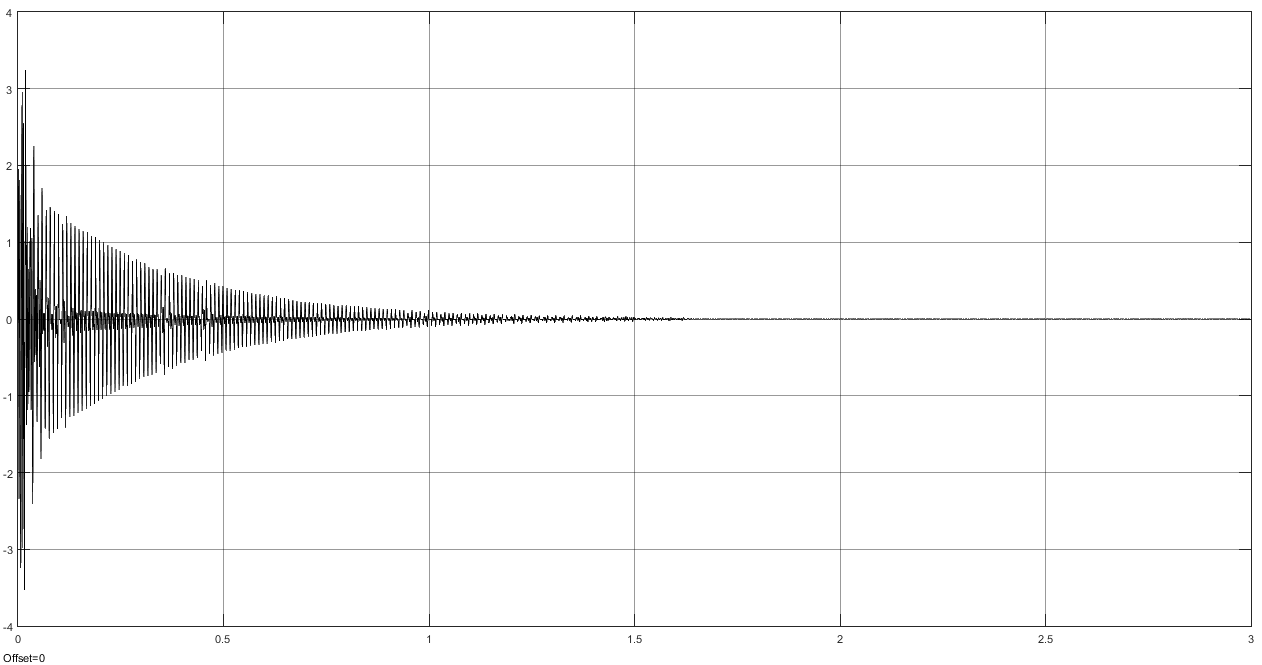
\includegraphics[width=\linewidth]{./pics/ResultadoPrimeiraOrdemEstimativaE0RefA.png}
  \captionof{figure}{Erro de Saída, Referência PE para um tempo finito}
  \label{fig:test60}
\end{minipage}
\end{frame}
\begin{frame}
\frametitle{Estimativas dos Parâmetros da Planta}
\centering
\begin{minipage}{.48\textwidth}
  \centering
  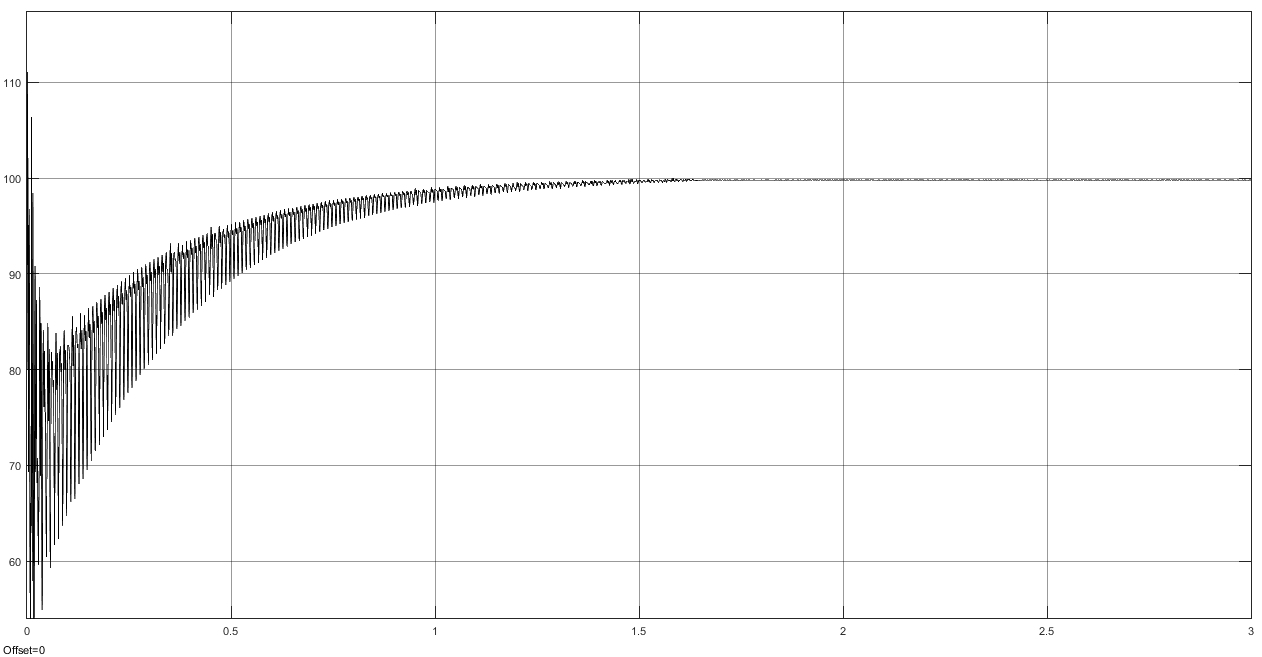
\includegraphics[width=\linewidth]{./pics/ResultadoPrimeiraOrdemEstimativaTheta1RefA.png}
  \captionof{figure}{Estimativa $\hat{\theta_1}$, $\theta_1^*=100$, Referência PE para um tempo finito}
  \label{fig:test70}
\end{minipage}%
  \hfill
\begin{minipage}{.48\textwidth}
  \centering
  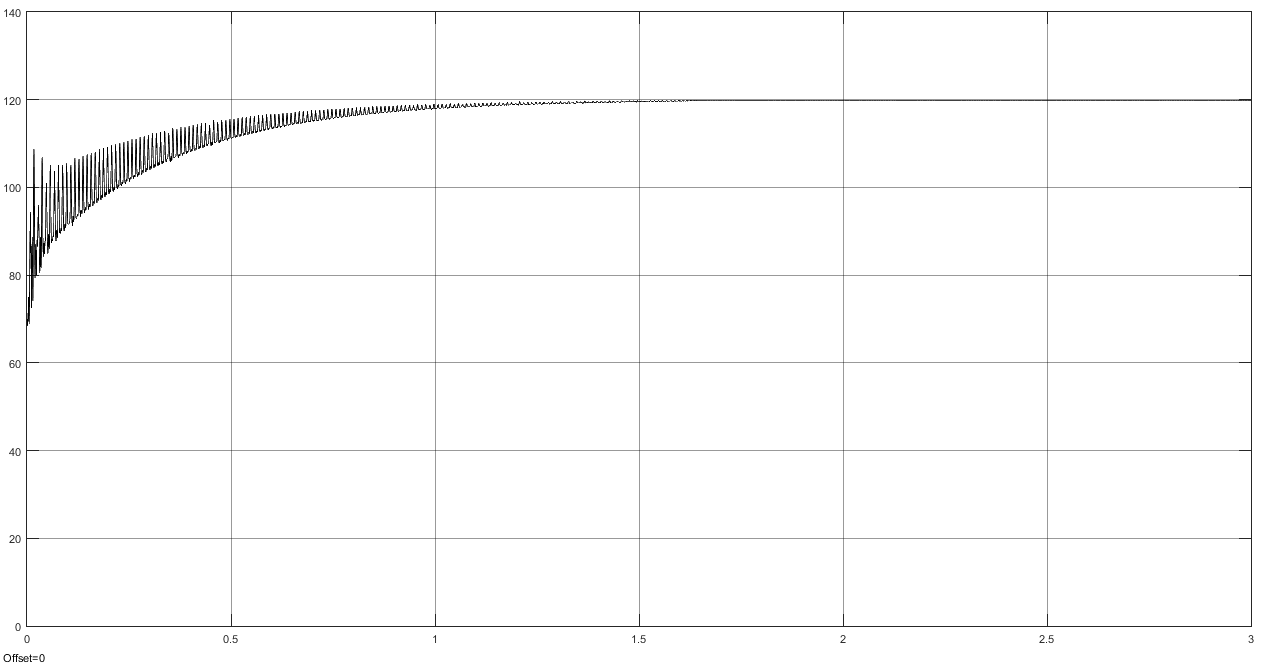
\includegraphics[width=\linewidth]{./pics/ResultadoPrimeiraOrdemEstimativaTheta2RefA.png}
  \captionof{figure}{Estimativa $\hat{\theta_2}$, $\theta_2^*=120$, Referência PE para um tempo finito}
  \label{fig:test80}
\end{minipage}
\end{frame}
% % % % % % % % % % % % % % % % % % % % % % % % % % % % % % % % % % %

\subsection{Planta de Segunda Ordem}% % % % % % % % % % % % % % % % %REF C
\begin{frame}
\frametitle{Sinal introduzido na Planta e Saída da Planta}
\centering
\begin{minipage}{.48\textwidth}
  \centering
  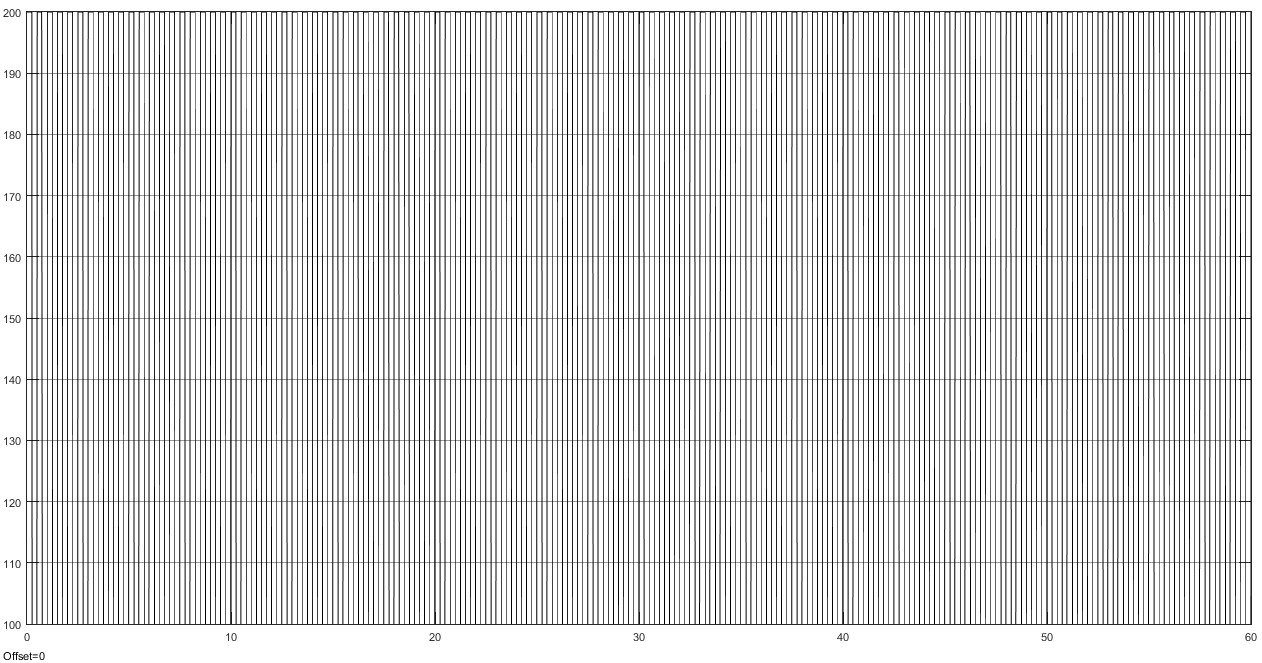
\includegraphics[width=\linewidth]{./pics/EntradaUSegOrdemRefC.png}
  \captionof{figure}{Sinal Introduzido na Planta, Referência PE para todo t}
  \label{fig:test311}
\end{minipage}%
  \hfill
\begin{minipage}{.48\textwidth}
  \centering
  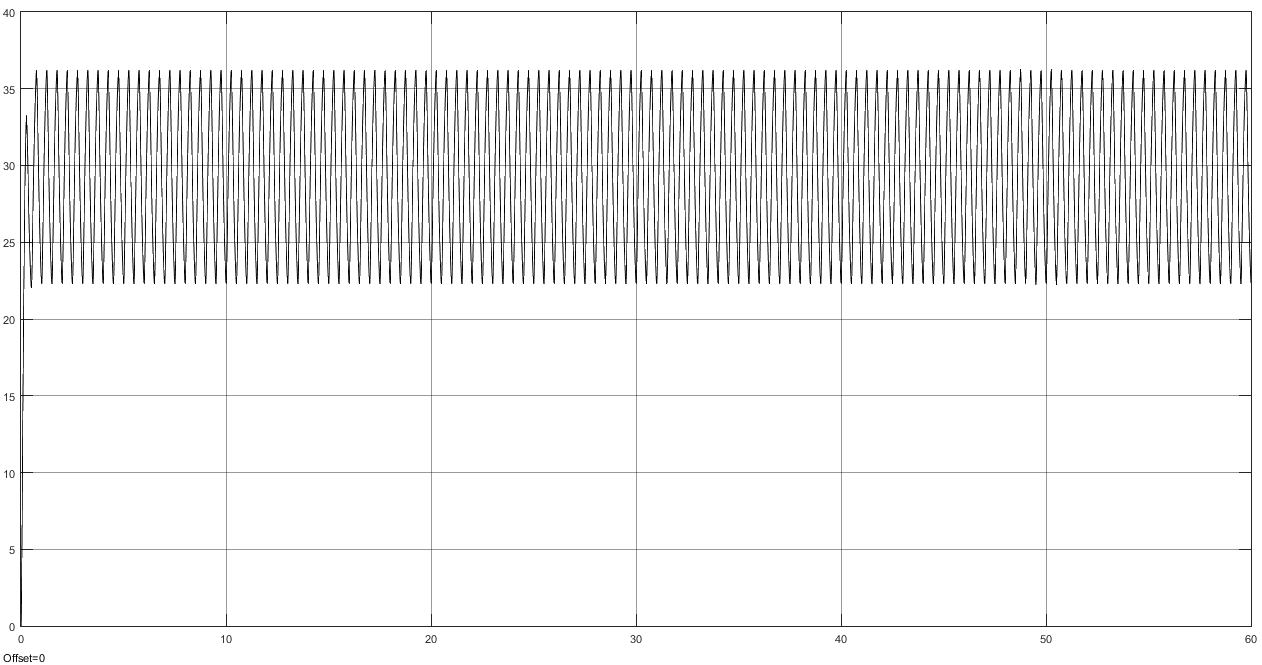
\includegraphics[width=\linewidth]{./pics/ResultadoSegundaOrdemEstimativaYRefC.png}
  \captionof{figure}{Saída da Planta, Referência PE para todo t}
  \label{fig:test411}
\end{minipage}
\end{frame}
\begin{frame}
\frametitle{Saída do Modelo da Planta e Erro de Saída}
\centering
\begin{minipage}{.48\textwidth}
  \centering
  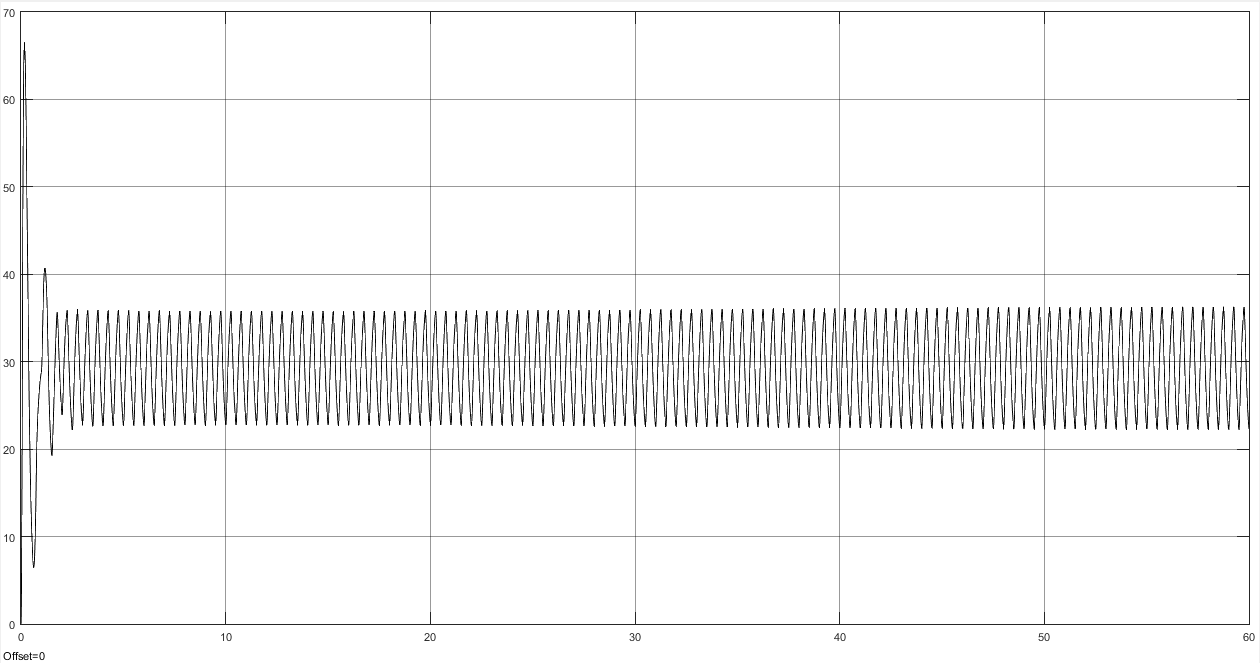
\includegraphics[width=\linewidth]{./pics/ResultadoSegundaOrdemEstimativaYcRefC.png}
  \captionof{figure}{Saída do Modelo da Planta, Referência PE para todo t}
  \label{fig:test51}
\end{minipage}%
  \hfill
\begin{minipage}{.48\textwidth}
  \centering
  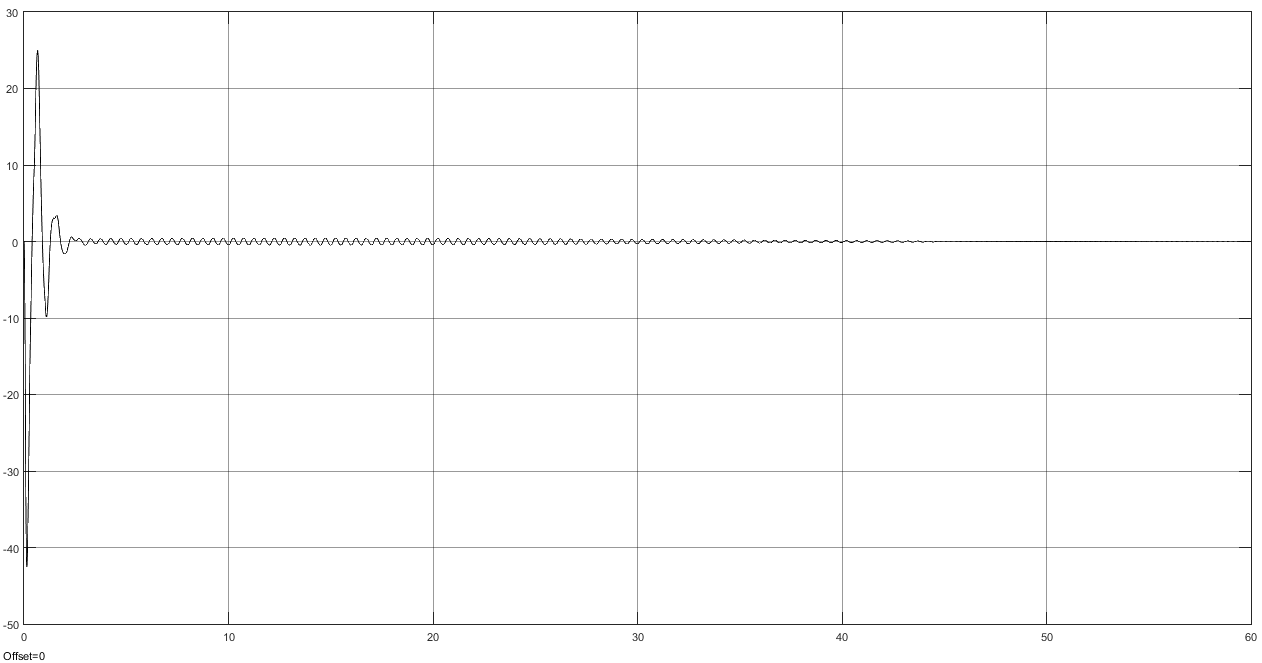
\includegraphics[width=\linewidth]{./pics/ResultadoSegundaOrdemEstimativaE0RefC.png}
  \captionof{figure}{Erro de Saída, Referência PE para todo t}
  \label{fig:test61}
\end{minipage}
\end{frame}
\begin{frame}
\frametitle{Estimativas dos Parâmetros da Planta}
\centering
\begin{minipage}{.48\textwidth}
  \centering
  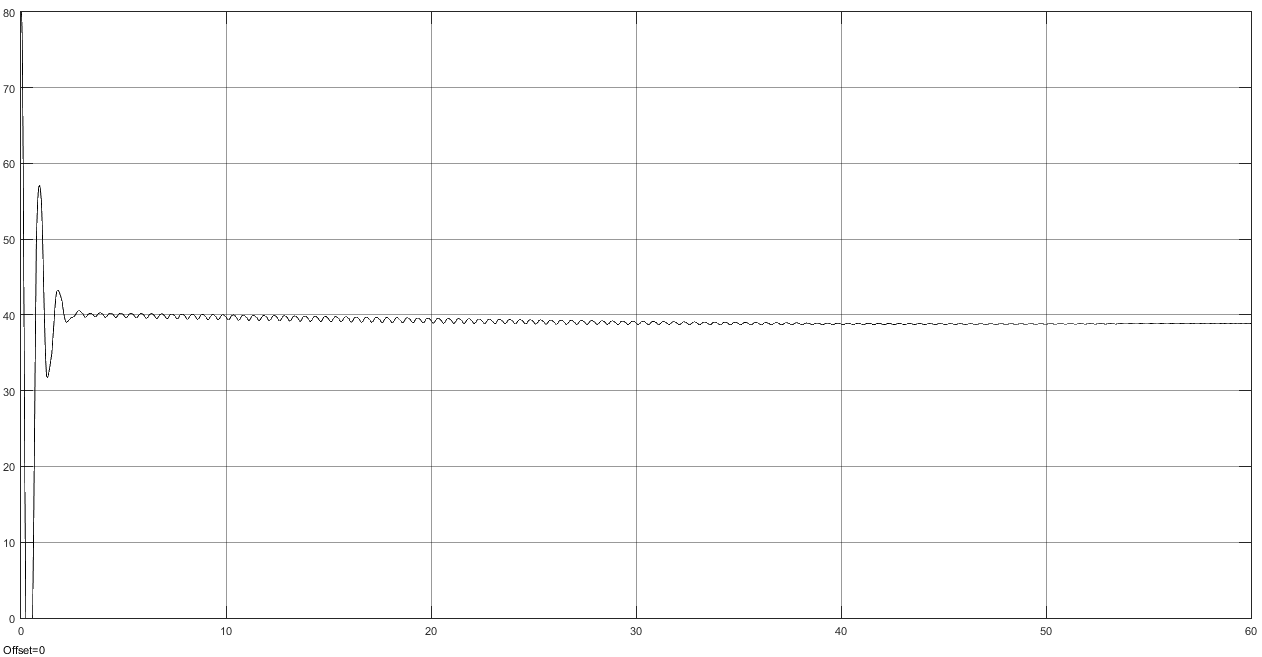
\includegraphics[width=\linewidth]{./pics/ResultadoSegundaOrdemEstimativaTheta1RefC.png}
  \captionof{figure}{Estimativa $\hat{\theta_1}$, $\theta_1^*=39$, Referência PE para todo t}
  \label{fig:test71}
\end{minipage}%
  \hfill
\begin{minipage}{.48\textwidth}
  \centering
  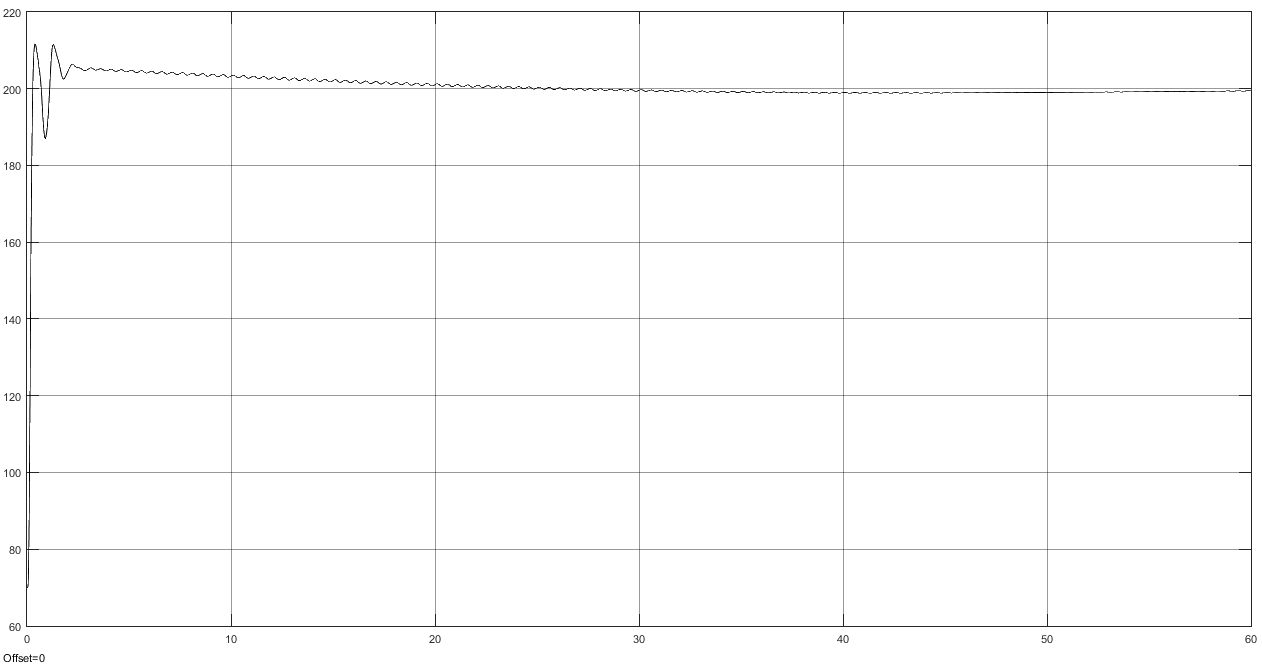
\includegraphics[width=\linewidth]{./pics/ResultadoSegundaOrdemEstimativaTheta2RefC.png}
  \captionof{figure}{Estimativa $\hat{\theta_2}$, $\theta_2^*=200$, Referência PE para todo t}
  \label{fig:test81}
\end{minipage}
\end{frame}

\begin{frame}
\frametitle{Planta de Segunda Ordem}
  \centering
  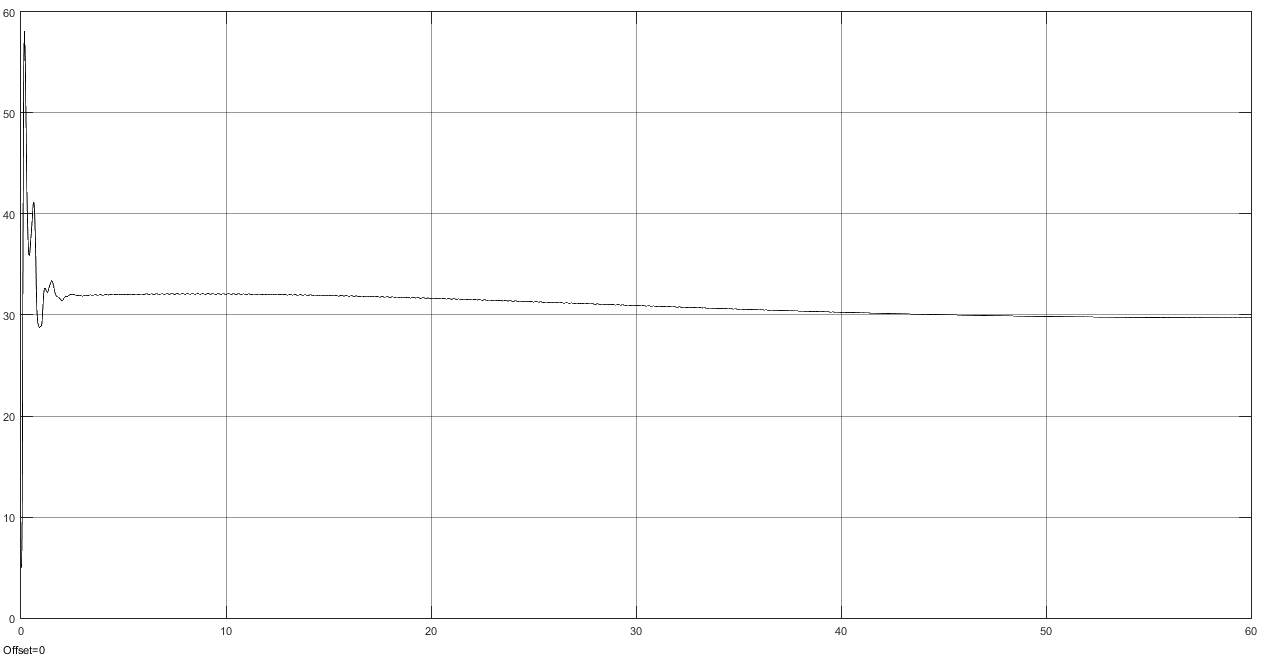
\includegraphics[width=.5\linewidth]{./pics/ResultadoSegundaOrdemEstimativaTheta3RefC.png}
  \captionof{figure}{Estimativa $\hat{\theta_3}$, $\theta_3^*=30$, Referência PE para todo t}
  \label{fig:test341}
\end{frame}


% % % % % % % % % % % % % % % % % % % % % % % % %REF A

\begin{frame}
\frametitle{Sinal introduzido na Planta e Saída da Planta}
\centering
\begin{minipage}{.48\textwidth}
  \centering
  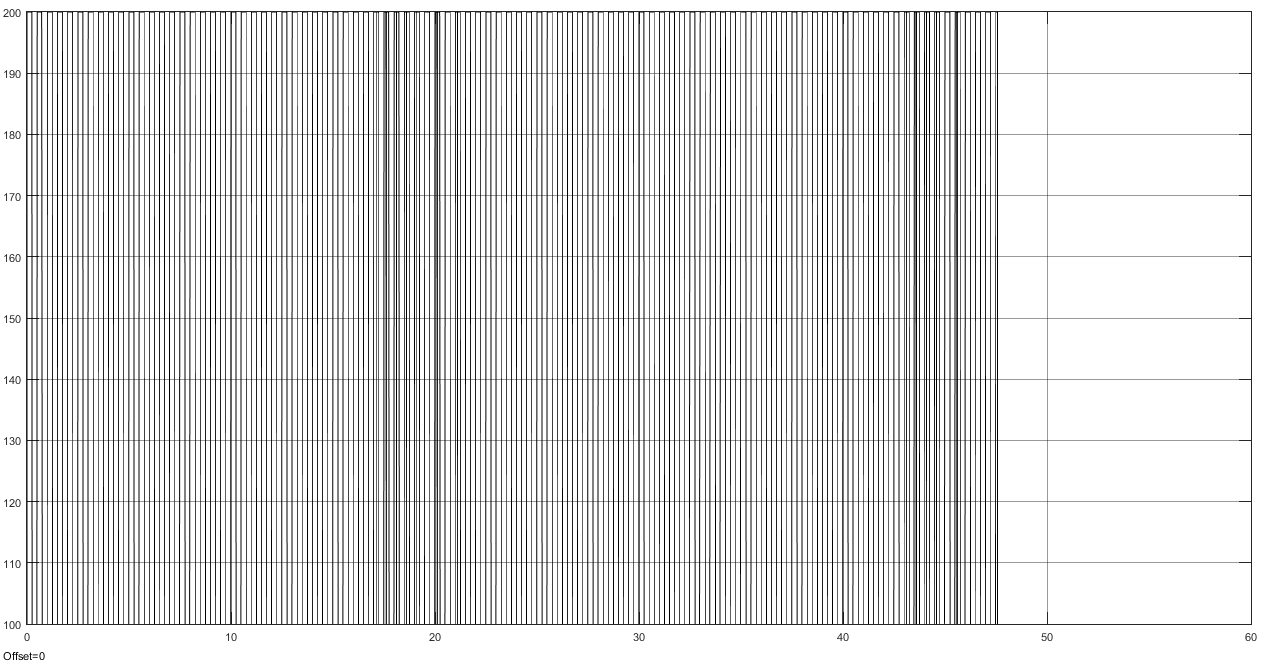
\includegraphics[width=\linewidth]{./pics/EntradaUSegOrdem.png}
  \captionof{figure}{Sinal Introduzido na Planta, Referência PE um tempo finito}
  \label{fig:test371}
\end{minipage}%
  \hfill
\begin{minipage}{.48\textwidth}
  \centering
  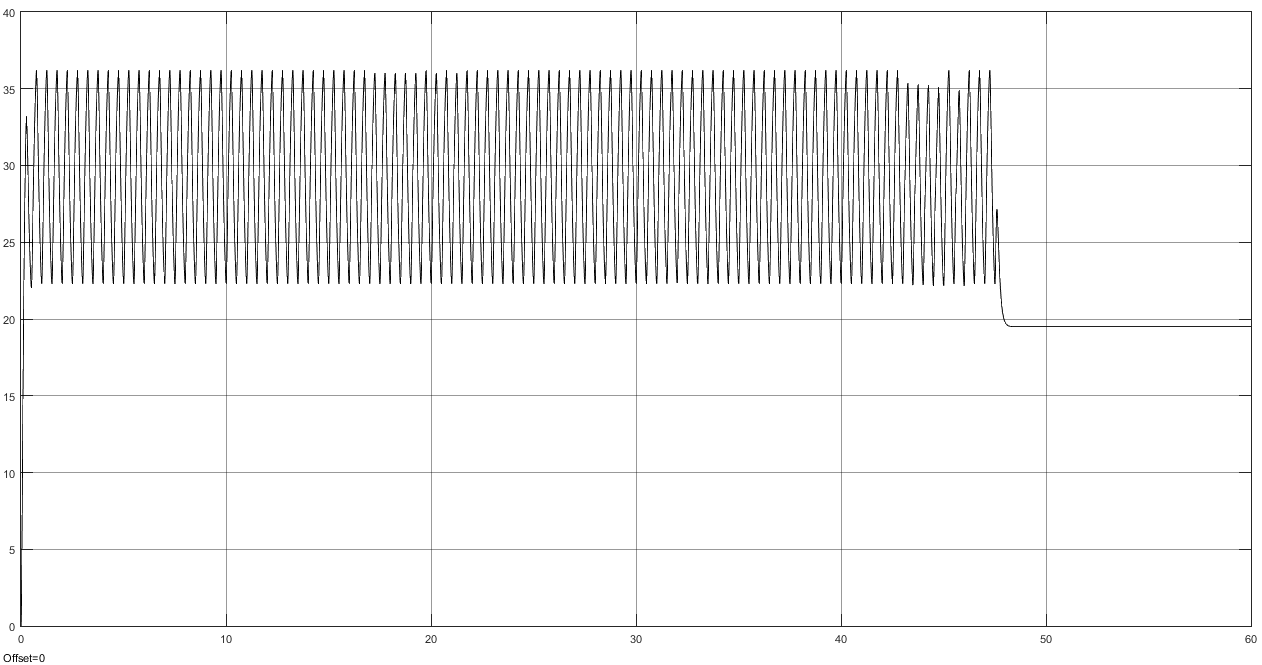
\includegraphics[width=\linewidth]{./pics/ResultadoSegundaOrdemEstimativaYRefA.png}
  \captionof{figure}{Saída da Planta, Referência PE para um tempo finito}
  \label{fig:test401}
\end{minipage}
\end{frame}
\begin{frame}
\frametitle{Saída do Modelo da Planta e Erro de Saída}
\centering
\begin{minipage}{.48\textwidth}
  \centering
  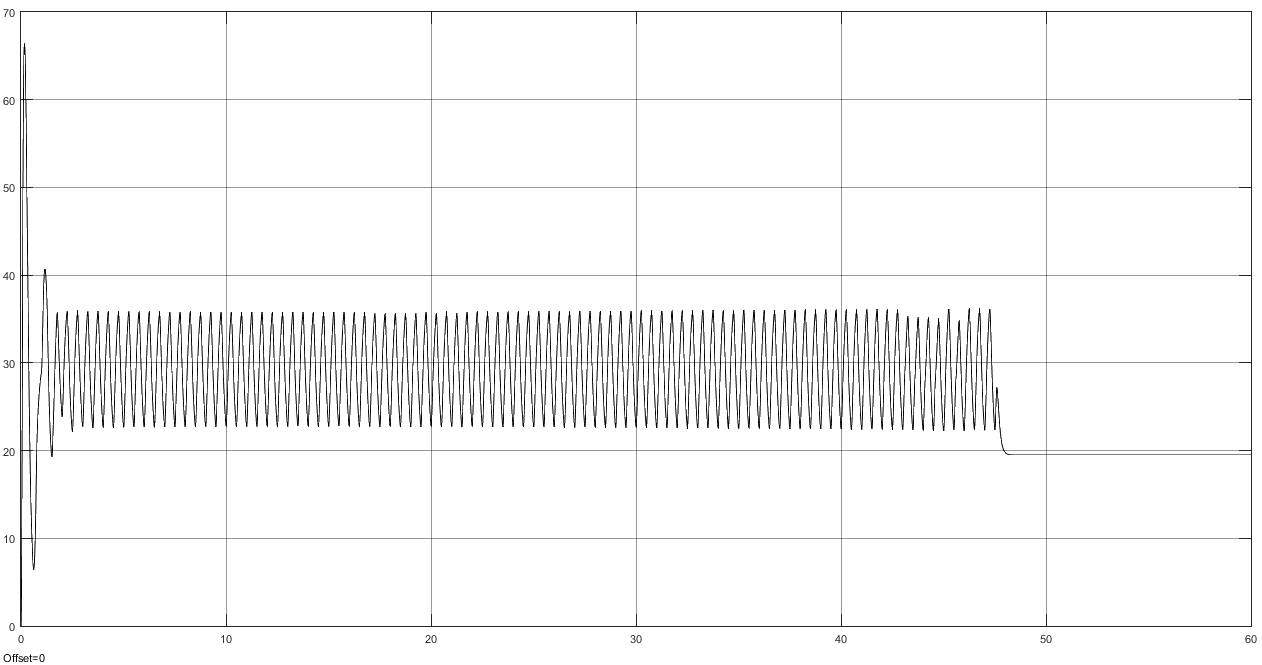
\includegraphics[width=\linewidth]{./pics/ResultadoSegundaOrdemEstimativaYcRefA.png}
  \captionof{figure}{Saída do Modelo da Planta, Referência PE para um tempo finito}
  \label{fig:test501}
\end{minipage}%
  \hfill
\begin{minipage}{.48\textwidth}
  \centering
  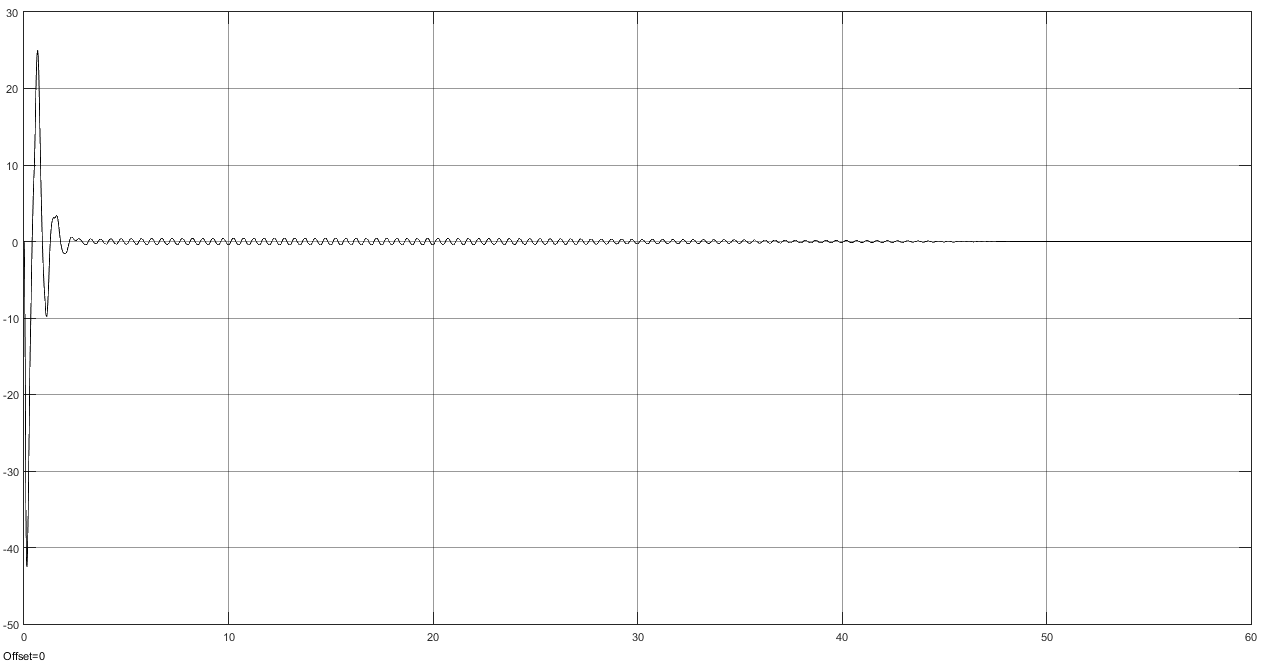
\includegraphics[width=\linewidth]{./pics/ResultadoSegundaOrdemEstimativaE0RefA.png}
  \captionof{figure}{Erro de Saída da Planta, Referência PE para um tempo finito}
  \label{fig:test601}
\end{minipage}
\end{frame}
\begin{frame}
\frametitle{Estimativas dos Parâmetros da Planta}
\centering
\begin{minipage}{.48\textwidth}
  \centering
  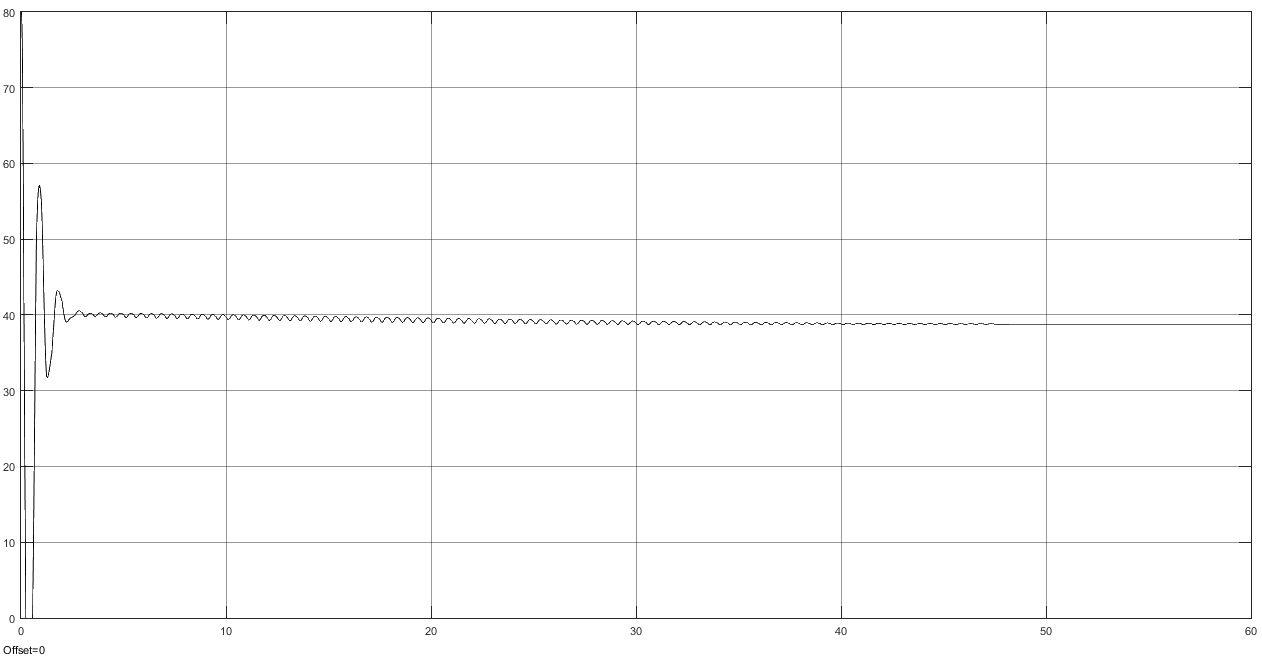
\includegraphics[width=\linewidth]{./pics/ResultadoSegundaOrdemEstimativaTheta1RefA.png}
  \captionof{figure}{Estimativa $\hat{\theta_1}$, $\theta_1^*=39$, Referência PE para um tempo finito}
  \label{fig:test701}
\end{minipage}%
  \hfill
\begin{minipage}{.48\textwidth}
  \centering
  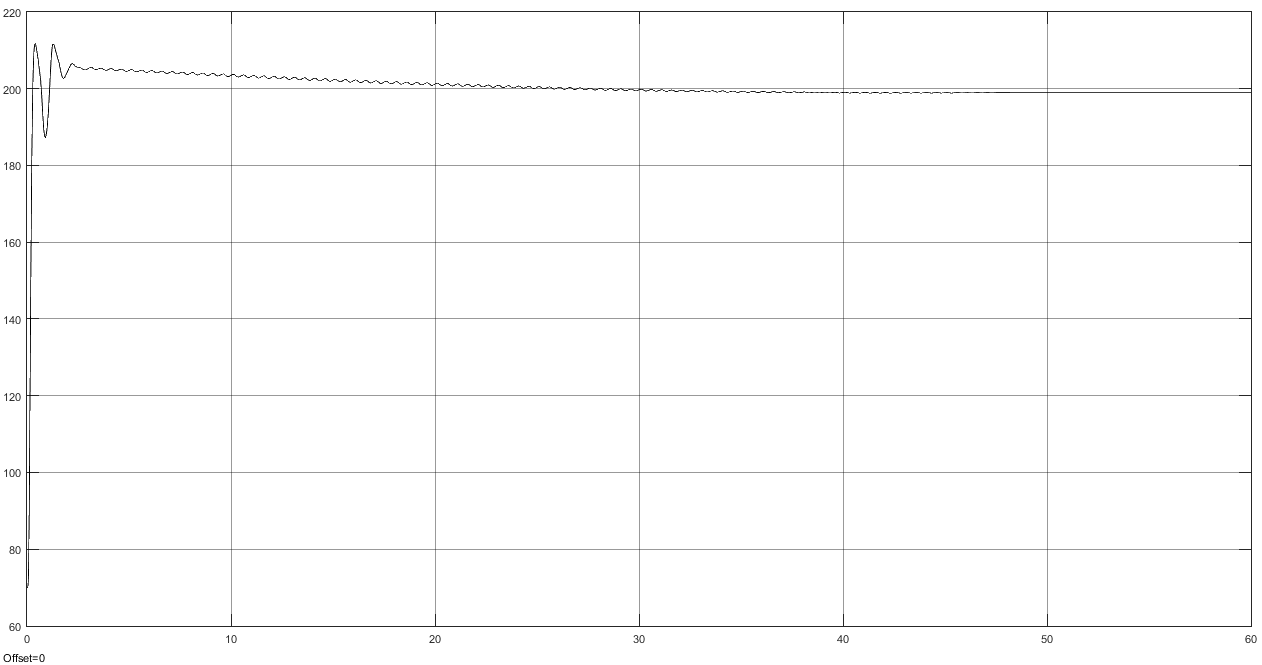
\includegraphics[width=\linewidth]{./pics/ResultadoSegundaOrdemEstimativaTheta2RefA.png}
  \captionof{figure}{Estimativa $\hat{\theta_2}$, $\theta_2^*=200$, Referência PE para um tempo finito}
  \label{fig:test801}
\end{minipage}
\end{frame}


\begin{frame}
\frametitle{Planta de Segunda Ordem}
  \centering
  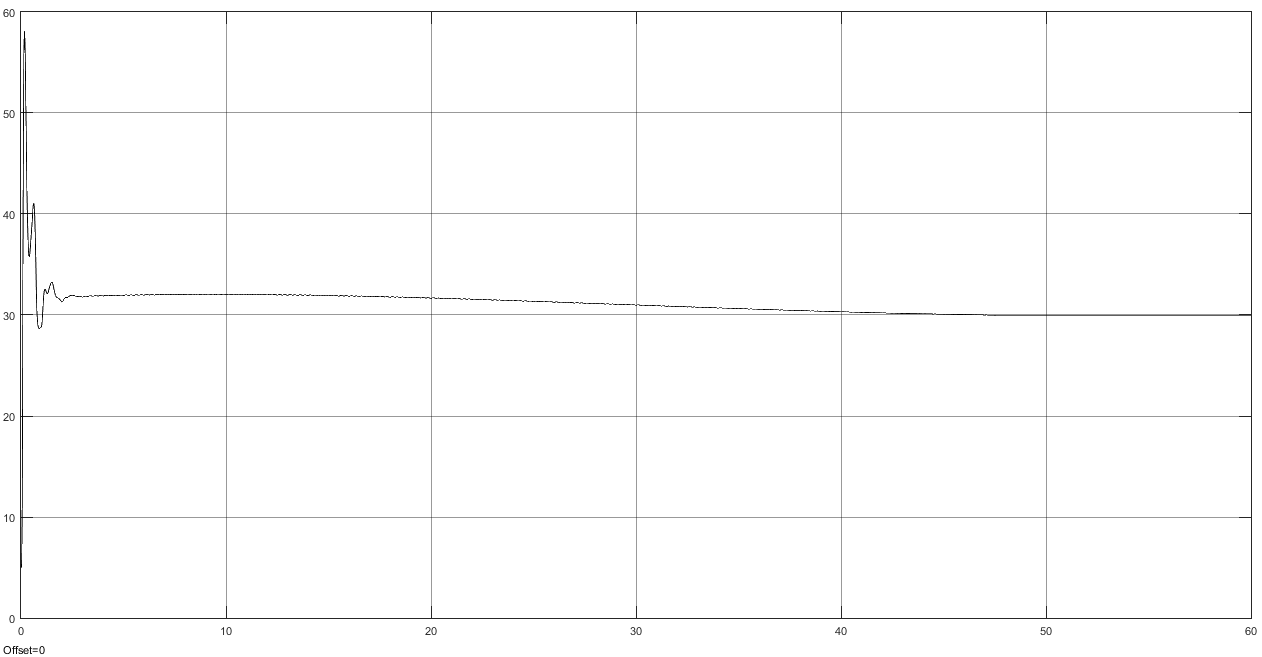
\includegraphics[width=.5\linewidth]{./pics/ResultadoSegundaOrdemEstimativaTheta3RefA.png}
  \captionof{figure}{Estimativa $\hat{\theta_3}$, $\theta_3^*=30$, Referência PE para um tempo finito}
  \label{fig:test3411}
\end{frame}

% % % % % % % % % % % % % % % % % % % % % % % % % % % % % % % % % % %

% ----------------- NOVO SLIDE --------------------------------
\section{Comentários Finais}
\subsection{Comentários Finais e Referências}

% --- O comando \allowframebreaks ---
% Se o conteúdo não se encaixa em um quadro, a opção allowframebreaks instrui 
% beamer para quebrá-lo automaticamente entre dois ou mais quadros,
% mantendo o frametitle do primeiro quadro (dado como argumento) e acrescentando 
% um número romano ou algo parecido na continuação.

\begin{frame}
\frametitle{Comentários Finais}
\begin{enumerate}
\item<1-> Estratégias de Controle\\
\item<2-> Detecção de Convergência dos Parâmetros\\ 
\item<3-> Ruídos e Perturbações Não Determinísticas\\
\item<4-> Variação dos Parâmetros da Planta no Tempo\\
\item<5-> Plantas Reais\\
\end{enumerate}

\end{frame}
% --- O comando \allowframebreaks ---
% Se o conteúdo não se encaixa em um quadro, a opção allowframebreaks instrui 
% beamer para quebrá-lo automaticamente entre dois ou mais quadros,
% mantendo o frametitle do primeiro quadro (dado como argumento) e acrescentando 
% um número romano ou algo parecido na continuação.

\begin{frame}[allowframebreaks]
\frametitle{Referências}
\bibliography{bib-controleadaptativo}
\nocite{ioannou2}
\nocite{chen}
\nocite{ogata}
\nocite{naval}
\nocite{ljung}
\nocite{aguirre}
\nocite{khalil}
\end{frame}
% ----------------- FIM DO DOCUMENTO -----------------------------------------
\end{document}
